\documentclass{article}


\usepackage[utf8]{inputenc}
\usepackage[a4paper, total={6in, 9in}]{geometry}
\usepackage{braket}
\usepackage{xcolor}
\usepackage{amsmath}
\usepackage{amsfonts}
\usepackage{tikz}
\usepackage{svg}
\usepackage{graphicx}
\usepackage{media9}
\usepackage{float}
\usetikzlibrary{calc}
\usepackage{array}
\usepackage[ruled,vlined,linesnumbered]{algorithm2e}

\usepackage[
backend=biber,
style=alphabetic,
sorting=ynt
]{biblatex}



\newcommand{\commentt}[1]{\textcolor{blue}{ \textbf{[COMMENT]} #1}}
\newcommand{\ctt}[1]{\commentt{#1}}
\newcommand{\prb}[1]{ \mathbf{Pr} \left[ {#1} \right]}
\newcommand{\onotation}[1]{\(\mathcal{O} \left( {#1}  \right) \)}
\newcommand{\ona}[1]{\onotation{#1}}
\newcommand{\nvar}[2]{ \( #1_{1}, #1_{2} ... #1_{#2}  \) }
%\newenvironment{proof}[0]{\paragraph{Proof.}}{}
%\newenvironment{remark}[0]{\textit{remark}}{}
\newenvironment{cor}[0]{\paragraph{Corollary.}}{}
\newenvironment{example}[0]{\paragraph{Example.}}{}
%\newenvironment{thm}[0]{\paragraph{Theorem.}}{}
\newtheorem{prop}{Proposition}
\newtheorem{ex}{Exercise}
\newtheorem{sol}{Solution}
\newtheorem{theorem}{Theorem} 		
\newtheorem{thm}{Theorem}[section]
\newtheorem{conj}[thm]{Conjecture} 	
\newtheorem{lemma}[thm]{Lemma}
\newtheorem{corollary}[thm]{Corollary} 
\newtheorem{claim}[thm]{Claim}
\newtheorem{proposition}[thm]{Proposition}
\newtheorem{definition}{Definition} 
\newtheorem{remark}{Remark}
 


% \addbibresource{sample.bib} %Import the bibliography file
\begin{document}    
\maketitle
\newcommand*{\RECITATION}{}%
\begin{document}
\chapter{Induction and Asymptotic Notations.}
Computer science differs from other scientific disciplines in that it focuses not on solving or making discoveries, but on questioning how good is our current understanding. The fact that one has successfully come up with an idea for a certain problem immediately raises the question of optimality. At the most basic level, we would like to answer what is the 'best' \marginnote[Note 1: text for left-hand side text]{Note 1: text for right-hand side of pages, it is set justified.} program that exists for a particular problem. To do so, we must have a notation that allows us to determine if an algorithm is indeed solving the task, quantify its performance, and compare it to other algorithms. In this chapter, we introduce this basic notation. The chapter is divided into two main parts: the first is about induction, a mathematical technique for proving claims, and the second presents asymptotic notation, which we use to describe the behavior of algorithms over large inputs.
 

% \section{Time Planning.}
% \begin{enumerate}
%     \item Welcome words, general information, listing the recitation topics \& QA. 7\textbf{m} (section 1).
%     \item Explain (remind) induction and presenting the first first example. 10\textbf{m}.
%     \item Second weak induction example 4\textbf{m}.
%     \item Strong induction 7\textbf{m}.
%     \item Introduce, the big O. explain the object shortly, plot graphs. yet still not formal definitions. 7\textbf{m}.  
%     \item Shoot the definitions of the \(O, \Omega, \Theta\) at one. 7\textbf{m}.
%     \item 3\textbf{m} spare + break. 
%     \item Review again the asymptotic notations, with examples from section 4. Q\&A. 7\textbf{m}
%     \item Lemma 21 7\textbf{m}
%     \item Claim 22 7\textbf{m}
%     \item The claim beneath Claim 22 7\textbf{m}
%     \item Example 23 7\textbf{m} (should take more time, the above claims will pay the tax). 
%     \item Logarithmic Rules 7\textbf{m}. 
% \end{enumerate}
% \section{General Course Information.}
% \begin{enumerate}
%     \item Introduce yourself
%     \item course mail: huji.dast.2022a@gmail.com
%     \item targilim scoring: 0.85 \( \cdot \) Test + 0.15 \( \cdot \) Average(\(N - 2\)). 
% \item  introduction to the course: \begin{enumerate}
%     \item  It’s important \& fun: \begin{enumerate}
%         \item We going to learn some data structures: Heaps, Trees, Hash Tables
%         \item And some algorithms: Sorting, Minimal Spanning Tree, Shortest Path
%     \end{enumerate}
%     \item Doing your homework by yourself is the best way to improve your solving problems skill.
% \end{enumerate}
% \end{enumerate}

% \paragraph{Abstract.} Today we will cover induction, infinite series, and asymptotic notation. These tools will come in handy (in the next couple of weeks) when we want to find the runtime complexity of an algorithm, specifically using the ’Master Theorem’, to give asymptotic bounds for recursion relations, and to prove loop invariants using (finite) induction.

\section{Induction.}
%Suppose that a teacher who standing in front of his class is willing to prove that he can reach the door. One obivieus way to do so is to actully reach the door, that's it, move physiclly to her and declere sucsses. For small classes contian small nummer of students that protcol even might be efficient,lasting less than servel secondes. But what if the class is really big one? mabye at the length and wide of a football stadium? In that case, the proving by doing might take time. So the obvious question to ask, what else can we do? is there more efficient way to prove that? 

%Suppose that a teacher, who's standing in front of his class, is willing to prove that he can reach the door at the corner. One obvious way to do so is to actually reach the door, that's it, move physically to it and declare success. For small classes containing a small number of students, this protocol might even be efficient, lasting less than several seconds. But what if the class is really big, maybe the length and width of a football stadium? In that case, the proving by doing might take time. So the obvious question to ask is, what else can we do? Is there a more efficient way to prove this?

Suppose that a teacher, who is standing in front of his class, is willing to prove that he can reach the door at the corner. One obvious way to do so is to actually reach the door; that is, move physically to it and declare success. For small classes containing a small number of students, this protocol might even be efficient, lasting less than several seconds. But what if the class is really big, maybe the length and width of a football stadium? In that case, proving by doing might take time. So the obvious question to ask is, what else can we do? Is there a more efficient way to prove this?

Indeed, there is. Instead of proving that he can reach the door, he can prove that while he do not stand next to the door, nothing can stop him from keeping moving forward. If that is indeed the case, then it's clear that not reaching the door in the end would be a contradiction to being just one step away from it (why?), which, in turn, would also contradict being two steps away from it. Repeating this argument leads to a contradiction for the fact that the teacher was in the classroom at the beginning.

\paragraph{What is induction?}~\begin{enumerate}
    \item A mathematical proof technique. It is essentially used to prove that a property \(P(n)\) holds for every natural number \(n\).
    \item The method of induction requires two cases to be proved:
    \begin{enumerate}
        \item The first case, called the base case, proves that the property holds for the first element.
        \item The second case, called the induction step, proves that if the property holds for one natural number, then it holds for the next natural number.
    \end{enumerate}
    \item The domino metaphor. 
\end{enumerate}

\begin{figure}[h]
  \centering
  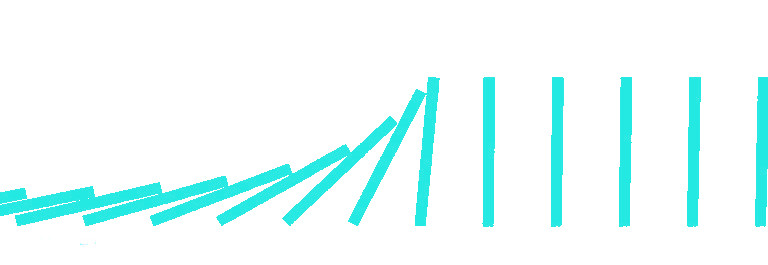
\includegraphics[scale=2]{./dommino-256x256}
  \caption{ domino line falling.}
  \label{fig:domino}
\end{figure}



\subsection{Two Types of Induction Strategies.}
We keep in mind two types of induction strategies: the first is Weak Induction, which refers to proofs that, in their step stage, only require assuming the correctness of the previous step, i.e. $P(n-1)$, in order to prove correctness for $P(n)$. This differs from the Strong Induction strategy, for which the step stage assumes the correctness of the claim for any value less than $n$, namely assuming that all $P(1), P(2), ..., P(n-1)$ are correct.


\Cref{example:chockstrong} and \Cref{example:sumweak2} demonstrate the use of weak induction to prove the formulas for arithmetic and geometric sums. \Cref{example:sumweak} uses strong induction to determine the number of splits required to separate a chocolate bar.

\begin{example}[Weak induction] 
  \label{example:sumweak}
Prove that $ \forall n \in  \mathbb{N}$: 
  \begin{equation*}
    \begin{split}
  \sum_{i=0}^{n}{i} = \frac{n(n+1)}{2}
    \end{split}
  \end{equation*}
  \begin{proof} By induction.
  \begin{enumerate}
    \item Base. For \(n = 1\), \(\sum_{i=0}^{1}{1} = 1 = \frac{(1+1)\cdot 1}{2} \). 
      \item Assumption. Assume that the claim holds for \(n\). 
      \item Step. 
\begin{equation*}
  \begin{split}
 \sum_{i=0}^{n+1}{i} = & \left( \sum_{i=0}^{n}{i} \right) + n+1 = \frac{n(n+1)}{2} + n + 1 \\
 = & \frac{n(n+1) + 2\cdot (n+1)}{2} = \frac{(n+1)(n+2)}{2} 
  \end{split}
\end{equation*}
  \end{enumerate}
\end{proof}
\end{example}
\begin{example}[Weak induction.] 
  \label{example:sumweak2}
  Let \(q\in \mathbb{R} / \{1\}\), consider the geometric series \( 1,q,q^2,q^3....q^k...\). Prove that the sum of the first \(k\) elements is \begin{equation*}
     1+q+q^2+...+q^{k-1}+q^k = \frac{q^{k+1}-1}{q-1}
\end{equation*}

\begin{proof} By induction. 
  \begin{enumerate}
    \item      Base. For \(n = 1\), we get \( \frac{q^{k+1}-1}{q-1} = \frac{q-1}{q-1} = 1\). 
    \item      Assumption. Assume that the claim holds for an integer \(k\). 
    \item      Step. 
      \begin{equation*}
	\begin{split}
	  1+q+q^2+... & + q^{k-1}+q^k + q^{k+1} =  \frac{q^{k}-1}{q-1} + q^{k+1}  \\
	  &= \frac{q^{k+1}-1 +q^{k+1}\left(q-1\right) }{q-1}  \\ &=\frac{\textcolor{red}{q^{k+1}}-1 +q^{k+2} - \textcolor{red}{q^{k+1}}  }{q-1} \\ &= \frac{q^{k+2}-1}{q-1} 
	\end{split}
      \end{equation*}
  \end{enumerate}
\end{proof}
\end{example}
% \ctt{Finish the induction proof and add alternative proof by counting. I am not sure what is favored, exposing both ways (at the first example) will make clear that induction is only a single proofing tool and surly not the only one. Yet from didactic point of view, it might confuses. }

\begin{example}[Strong induction] 
  \label{example:chockstrong}
  Let there be a chocolate bar that consists of \(n\) square chocolate blocks. Then it takes exactly \(n - 1\) snaps to separate it into the \(n\) squares no matter how we split it.

  \begin{proof} By strong induction. 
    \begin{enumerate}
      \item	Base. For \(n = 1\), it is clear that we need \(0\) snaps. 
      \item	Assumption. Assume correctness for \textbf{every} \(m < n \).
      \item	Step. We have in our hand the given chocolate bar with \(n\) square chocolate blocks. Then we may snap it anywhere we like, to get two new chocolate bars: one with some \( k \in [n]\) chocolate blocks and one with \(n - k\) chocolate blocks. From the induction assumption, we know that it takes \(k - 1\) snaps to separate the first bar, and \(n - k - 1\) snaps for the second one. And to sum them up, we got exactly \[ (k - 1) + (n - k - 1) + 1 = n - 1 \] snaps.
    \end{enumerate}
\end{proof}
\end{example}
\section{Asymptotic Notations.}


\begin{definition}
  Let \( f, g : \mathbb{N} \rightarrow \mathbb{R}^{+} \). We say that \( f(n) = O(g(n))\)  if \( \exists N \in \mathbb{N}, \exists c > 0 \) s.t. \( \forall n \ge N \ : \ f(n) \le c \cdot g(n)\). 
\end{definition}
\begin{example}
  For exmaple, if \(f(n) = n + 10 \) and \( g(n) = n^2\)
, then \(f(n) = O(g(n)) \) (Draw the graphs) for \(n \ge 5 \):
\(f(n) = n + 10 \le n + 2n = 3n \le n \cdot n = n^2\)
\end{example}
\begin{figure}[h]
  \label{fig:bigO}
\begin{tikzpicture}
    \draw[->]  (0,0)coordinate(O) -- (11,0) node[anchor=north] {$n$};
    \draw[->]  (0,0) -- (0,5);

    \draw[domain=0:6,smooth,variable=\x,blue,name path=c1] plot ({\x},{0.5*( (0.5*\x)^2+2*sin(\x r)+1)})node[right]{$f_1(n)$};
    \draw[domain=0:11,smooth,variable=\x,red,name path=c2] plot ({\x},{0.5*(0.2*\x+0.5*sin(\x r)+2)})node[right]{$f_2(n)$};
\fill[red,name intersections={of=c1 and c2}]
    (intersection-1) circle (2pt);

\draw[dashed] (intersection-1) -- (intersection-1|-O) node[below]{$N$};
\end{tikzpicture}
\end{figure}


\begin{definition} 
Let \( f, g : \mathbb{N} \rightarrow \mathbb{R} \)
We say that \(f(n) = \Omega(g(n))\) if \(g(n) = O(f(n))\), equivalently,
\( \exists N \in \mathbb{N}, \exists c > 0 \) s.t. \( \forall n \ge N c_0· g(n) \le f(n) \)
\end{definition}
\begin{example}
  Also if \( f(n) = 5n\) and \(g(n) = n^2\), then \(f(n) = O(g(n))\) (Now discuss intuition - no matter how much we “stretch” \(f, g\) is still the winner)
\end{example}

\begin{definition} 
Let \( f, g : \mathbb{N} \rightarrow \mathbb{R} \), We say that \(f(n) = \Omega(g(n))\) if:
\( \exists N \in \mathbb{N}, \exists c > 0 \) s.t \( \forall n \ge N \ f(n) \ge c \cdot g(n) \).
\end{definition}
\begin{example}
For exmaple, if \(f(n) = n + 10\) and \(g(n) = n^2\)
, then \(g(n) = \Omega(f(n))\)
\end{example}

\begin{figure}[h]
  \label{fig:bigTheta}
\begin{tikzpicture}
    \draw[->]  (0,0)coordinate(O) -- (11,0) node[anchor=north] {$n$};
    \draw[->]  (0,0) -- (0,5);

    \draw[domain=0:11,smooth,variable=\x,blue,name path=c1] plot ({\x},{0.5*( 0.5*\x+2*sin(\x r)+1)})node[right]{$f_1(n)$};
    \draw[domain=0:11,smooth,variable=\x,red,name path=c2] plot ({\x},{0.5*(0.2*\x+0.5*sin(\x r)+2)})node[right]{$f_2(n)$};
\fill[red,name intersections={of=c1 and c2}]
    (intersection-1) circle (2pt)
    (intersection-2) circle (2pt)
        (intersection-3) circle (2pt) ;

%\draw[dashed] (intersection-2) -- (intersection-2|-O) node[below]{n};
\end{tikzpicture}
\end{figure}


\begin{definition}
Let \( f, g : \mathbb{N} \rightarrow \mathbb{R} \), We say that \(f(n) = \Theta(g(n))\) if:
\(f(n) = O(g(n))\) and \(f(n) = \Omega(g(n))\)
That is, we say that \(f(n) = \Theta(g(n))\) if:
\( \exists N \in \mathbb{N}, \exists c_1, c_2 > 0\) s.t. \(\forall n \ge N \ c_1\cdot g(n) \le f(n) \le c_2 \cdot g(n)\)
\end{definition}
\begin{example} For every \(f : \mathbb{N} \rightarrow \mathbb{R}, f(n) = \Theta(f(n))\) \end{example}
\begin{example} If \(p(n) = n^5\) and \(q(n) = 0.5n^5 + n\), then \(p(n) = \Theta(q(n))\)\end{example}
But why is this example true? This next Lemma helps for intuition:
\begin{lemma}
  \( \lim_{n \rightarrow \infty} \frac{f(n)}{g(n)} < \infty \Rightarrow f(n) = O(g(n)) \)
\end{lemma}

\begin{proof} Assume that \(l = \lim_{n \rightarrow \infty} \frac{f(n)}{g(n)} < \infty\). Then for some \(N \in \mathbb{N}\) we have that for all \(n \ge N\):
\( \frac{f(n)}{g(n)} < l + 1 \Rightarrow f(n) < (l + 1) · g(n) \)
Which is exactly what we wanted.
\end{proof}
\section{Examples with proofs.}
% EXAMPLES WITH PROOFS

\begin{claim} \(n = O(2^n)\)
\end{claim}
(This must seem very silly, but even though we have a strong feeling it’s true, we still need to learn how to PROVE it)
\begin{proof} We will prove by induction that \( \forall n \ge 1 \) , \(2^n \ge n\), and that will suffice.
  \begin{enumerate}
    \item      Base. \(n = 1\), so it is clear that: \(n = 1 < 2 = 2^n\)
    \item      Assumption. Assume that \(n < 2^n\) for some \(n\).
    \item      Step. We will prove for \(n + 1\). It holds that:
      \begin{equation*}
	n + 1 < 2^{n} + 1 < 2^n + 2^n = 2^{n+1}
      \end{equation*}
  \end{enumerate}
\end{proof}
\begin{claim}
Let $p(n)$ be a polynomial of degree $d$ and let $q(n)$ be a polynomial
of degree $k$. Then:
\begin{enumerate}
\item $d\leq k\Rightarrow p(n)=O(q(n))$ (set upper bound over the quotient)
\item $d\geq k\Rightarrow p(n)=\Omega(q(n))$ (an exercise)
\item $d=k\Rightarrow p(n)=\Theta(g(n))$ (an exercise)
\end{enumerate}
\end{claim}
\begin{proof}Proof (Of 1) First, let's write down $p(n), g(n)$ explicitly:


% \begin{abstract}
%     Combinatorial Review, Induction, and Asymptotic Notations. 
% \end{abstract}
\[
p(n)=\sum_{i=0}^{d}\alpha_{i}n^{i},\ g(n)=\sum_{j=0}^{k}\beta_{j}n^{j}
\]
Now let's manipulate their quotient:
\[
\frac{p(n)}{q(n)}=\frac{\sum_{i=0}^{d}\alpha_{i}n^{i}}{\sum_{j=0}^{k}\beta_{j}n^{j}}=\frac{\sum_{i=0}^{d}\alpha_{i}n^{i}}{\sum_{j=0}^{k}\beta_{j}n^{j}}\cdot\frac{n^{k-1}}{n^{k-1}}=\frac{\sum_{i=0}^{d}\alpha_{i}n^{i-k+1}}{\sum_{j=0}^{k}\beta_{j}n^{j-k+1}}\leq
\]

\[
\leq\frac{\sum_{i=0}^{d}\alpha_{i}}{\beta_{k}} < \infty
\]
And now we can use the lemma that we have proved earlier. 
\end{proof}

\section{Logarithmic Rules.}

Just a quick reminder of logarithmic rules:
\begin{enumerate}
\item $log_{a}x\cdot y=log_{a}x+log_{a}y$
\item $log_{a}\frac{x}{y}=log_{a}x-log_{a}y$
\item $log_{a}x^{m}=m\cdot log_{a}x$
\item Change of basis: $\frac{log_{a}x}{log_{a}y}=log_{y}x$
\end{enumerate}
And so we get that:
\begin{remark}
For every $x,a,b\in\mathbb{R},$ we have that $log_{a}x=\Theta(log_{b}x)$
\end{remark}

\begin{example} Let \(f(n)\) be defined as:
\begin{equation*}
f(n) = \left\{ \begin{array}{rcl}
& f\left( \lfloor  \frac{n}{2} \rfloor \right) + 1 & \mbox{for }  n > 1  \\
& 5 & \mbox{else}  
\end{array}\right.
\end{equation*}
Let’s find an asymptotic upper bound for \(f(n)\). let's guess \( f(n) = O(\log(n)) \).

\begin{proof}  We’ll prove by strong induction that : \(f(n) < c \log(n) - 1\) for \(c =8 \) And that will be enough (why? This implies \(f(n) = O(\log(n))\)).
  \begin{enumerate}
    \item      Base. \(n = 2\). Clearly, \(f(2) = 6 < 8 \)
    \item      Assumption. Assume that for every m < n, this claim holds.
    \item      Step. Then we get:
      \begin{equation*} \begin{split}
	  f(n) &= f\left( \lfloor  \frac{n}{2} \rfloor \right) + 1 \le c\log\left(  \lfloor\frac{n}{2}\rfloor\right)  + 1  \\ & \le c\log\left(n\right) - c\log\left(2\right) + 1 
	  \le c\log\left(n\right) \ \ \ \text{for } c = 8
	\end{split}
      \end{equation*}
  \end{enumerate}
\end{proof}
\end{example}

% \section{Another Example.}


% Now let’s try to analyze something we’re going to encounter in this course: Recursively defined functions (Like Fibonacci’s
% sequence).


% \paragraph{Example 23.} Let \(f(n)\) be defined as:
% \begin{equation*}
% f(n) = \left\{ \begin{array}{rcl}
% & 2f\left( \lfloor  \frac{n}{2} \rfloor \right) + 1 & \mbox{for }  n > 1  \\
% & 1 & \mbox{else}  
% \end{array}\right.
% \end{equation*}
% Let’s find an asymptotic upper bound for \(f(n)\).
% We can unravel this recursion rule, and to make things easier let’s just assume that n is a power of 2. So we get:
%     \begin{equation*}
%     f(n) = 2f\left(\frac{n}{2}\right) + 1 =2\left(2f\left(\frac{n}{4}\right) + 1\right) + 1 = ... = nf(1)+ \left( n -1 \right) = 2n-1
%     \end{equation*}

% Proof. \textbf{(Bad proof)}
% Proof by strong induction. We’ll try to prove using \(N = 1, c = 10\), and we’ll try to show that \(f(n) < c \cdot n\).
% Base: \(n = 1\). Clearly we get that \(f(1) = 1 < 10 = c \cdot 1\)

% Assumption: Assume that for every \(m < n\), this claim holds.
% Step: We get:
% \begin{equation*}
%     f(n) = 2f\left( \lfloor  \frac{n}{2} \rfloor \right) + 1 \le 2c\lfloor  \frac{n}{2} \rfloor  + 1 \le c\cdot n + 1
% \end{equation*}
% But this is not a proof... (why? Didn’t prove hypothesis)


% Proof. \textbf{(Good proof)} We’ll try to prove something a little different. We’ll prove by strong induction that (with the same \(N, c\) ): \(f(n) < c \cdot n - 1\) And that will be enough (why? This implies \(f(n) = O(n)\)).
% Base: \(n = 1\). Clearly, \(f(1) = 1 < 9 = c \cdot 1 - 1\)
% Assumption: Assume that for every m < n, this claim holds.
% Step: Then we get:
% \begin{equation*}
%     f(n) = 2f\left( \lfloor  \frac{n}{2} \rfloor \right) + 1 \le 2\left(c  \frac{n}{2} -1 \right)  + 1 \le c\cdot n - 1
% \end{equation*}

% Remark 24. Note that in the definition of big \(O\) notation (12), the property only needs to hold from some \(N\) and on. In this
% last proof, we chose that \(N\) to be \(N = 1\), but it does not has to be 1.


% \section{SERIES AND CONVERGENCE.}

% \paragraph{Definition 3.} Let \( \{a_n\}^{\infty}_{n = N} \) be a sequence of real number. The sequence of partial sums corresponding to this sequence is \(S_k = \sum^{k}_{n=N}{a_n} \) an which is also a sequence of real numbers, with indices ranging from \(N\) to \(\infty\).
% \paragraph{Definition 4.} Let \( \{a_n\}^{\infty}_{n=N} \) be a sequence of real number. We say that the infinite series \( \sum^{\infty}_{n=N}{a_n} \)  converges when the sequence of partial sums converges, i.e. \(S_{k \rightarrow \infty} \rightarrow L \in \mathbb{R} \). In which case we say \( \sum^{\infty}_{n=N}{a_n} = L \). Otherwise, we say it diverges.

% Remark 5. Note that we can always ’pad’ the series with zeros, and this does not alter its convergence status. So we shall talk about series which their initial index is zero (or one).
% \paragraph{Example 6.} The Harmonic series \( \sum^{\infty}_{n=1}{\frac{1}{n}}\) diverges.

% Proof. Assume by contradiction it doesn’t, then there is a bound \( \lim_{k\rightarrow \infty} S_k = S \in \mathbb{R} \). So \(\lim_{k\rightarrow \infty} S_{2k} = S \in  R \). Thus \( \lim_{k} S_{2k}-S_{k} = 0 \), but \( S_{2k}-S_{k} = \frac{1}{n+1} + ... + \frac{1}{2n} \ge n \cdot \frac{1}{2n} = \frac{1}{2} \)
% , which is a contradiction, as we assumed \( \lim_{k\rightarrow \infty} S_{2k}-S_{k} = 0 \).

% \paragraph{Proposition 7.} If \( \{ S_k \}^{\infty}_{n=0} \) an converges, then \( a_{n\rightarrow\infty} \rightarrow 0 \). Proof. Consider \( \lim_{n\rightarrow\infty} [S_{n} - S{_n-1}]\).

% \paragraph{Example 8.} Let \(a_{n}= q^n\) be a sequence of real numbers, \(q \in \mathbb{R}\).
% \begin{enumerate}
%     \item If \(q < 1\), then \(S_k\) converges.
%     \item If \( q \ge 1\), then \(S_k\) diverges.
% \end{enumerate}
% Proof.
% \begin{enumerate}
%     \item Note that \[(1-q)S_{k} = \left(1-q\right)\left(1 + q + q^2 .. q^k \right) = \left(1 + q + q^2 + .. + q^k - q - q^2 - .. - q^{k+1} \right) = 1 - q^{k+1}   \] therefore \(S_k = \frac{1-q^{k+1}}{1-q} \), which    converges for \(k \rightarrow \infty \). That is \( S_k \rightarrow \frac{1}{1-q} \).
%     \item Exercise.
% \end{enumerate}
% \subsection{Convergence Tests}
% \paragraph{Theorem 9.} (Direct Comparison Test) Let \( \{a_n\}^{\infty}_{n = N} \),\( \{b_n\}^{\infty}_{n = N} \) be real, non-negative sequences, and assume \( \exsits M \in \mathbb{N}\) s.t. \( \forall n \ge M\), \( a_n \le b_n\). Then:
% \begin{enumerate}
%     \item If \(\sum^{\infty}_{n=1}{b_n}\) converges, so does \(\sum^{\infty}_{n=1}{a_n}\).
%     \item If \(\sum^{\infty}_{n=1}{a_n}\) diverges, so does \(\sum^{\infty}_{n=1}{b_n}\).
% \end{enumerate}


% Proof. Exercise (Guidance: Show that the partial sums corresponding to the sequence \(b_n\) are larger than the partial sums
% corr. to \(a_n\), and use a result from Infi about limits).

% \paragraph{Theorem 10.} (Limit comparison Test, generalized) Let \( \{a_n\}^{\infty}_{n = N} \),\( \{b_n\}^{\infty}_{n = N} \) be real, non-negative sequences,
% and assume \( \exsits M \in \mathbb{N}, r > 0, R > 0 \)  s.t \( \forall n \ge M, r \le \frac{a_n}{b_n} \le R\). Then either \( \sum_{n=1}^{\infty}{a_n} \)
% and \( \sum_{n=1}^{\infty}{b_n} \) both converge or they both diverge.
% Proof. Use the previous theorem (direct comparison) with \(rb_n \le a_n \le Rb_n\) along with limit arithmetics.

% \paragraph{Example 11.} \( \sum_{n=1}^{\infty}{\frac{1}{n^2}} \) converges.
% Proof. Note that \( \frac{1}{n^2} \le \frac{1}{n(n-1)} \), so it is enough to prove that the series 
% \( \sum_{n=2}^{\infty}{\frac{1}{n(n-1)}}\) converges by Direct Comparison. Notice that the partial sums are:
% \begin{equation*}
%     S_k = \sum_{n=2}^{k}{\frac{1}{n(n-1)}} = \sum_{n=2}^{k}{\frac{1}{n-1} - \frac{1}{n}} = \\ \left(1 - \frac{1}{2} \right) + \left( \frac{1}{2} - \frac{1}{3} \right) + ... + \left( \frac{1}{k-1} - \frac{1}{k} \right) = \\ 1 - \frac{1}{k}   
% \end{equation*}
% so the sequence of partial sums clearly converges (to 1).
% Proof. (Alternative) Look at the sides of the squares. We could always fit one more line of 2
% k
% squares for elements 2
% k until 2
% k+1 − 1 of the
% series. The total area of the rect angle here is 2.



% \printbibliography 
\end{document}
